%! Author = joels
%! Date = 13/07/2021

\section{Angular}
Flexible SPA Framework for CRUD applications: Typescript 4.1 based, Reduces boilerplate Code, DI Mechanism, JS-optimized 2-way binding, Clearly structured, information hiding, Increases testability / maintainability of client-side code\\
\textcolor{b}{\textbf{ngModules:}} Cohesive block of code dedicated to closely related set of capabilities. (\textit{module})
\textcolor{b}{\textbf{Directives:}} Provides instructions to transform the DOM. (\textit{class})
\textcolor{b}{\textbf{Components:}} Directive-with-a-template; it controls a section of the view. (\textit{class})
\textcolor{b}{\textbf{Templates:}} Form of HTML defining how to render the component. (\textit{HTML/CSS})
\textcolor{b}{\textbf{Metadata:}} Describes a class and defines how to process it. (\textit{decorator})
\textcolor{b}{\textbf{Services:}} Provides logic of any value, function or feature that the app needs. (\textit{class})
\subsection{Angular Modules (ngModule)}
Base for Angular modularity system. Every app has at least one Module, the root Module (a.k.a app Module). Root Module ist launched to bootstrap the app. Modules export features (directives, services) required by other modules.\\
\textcolor{b}{\textbf{TypeScript Module vs. ngModule:}}\\
ngModule is a logical block of multipe TypeScript modules linked together. The ngModule declaration itself is placed into a TypeScript module. Modules can accommodate sub-modules. All public TS members are exported as an overall \textit{barrel}
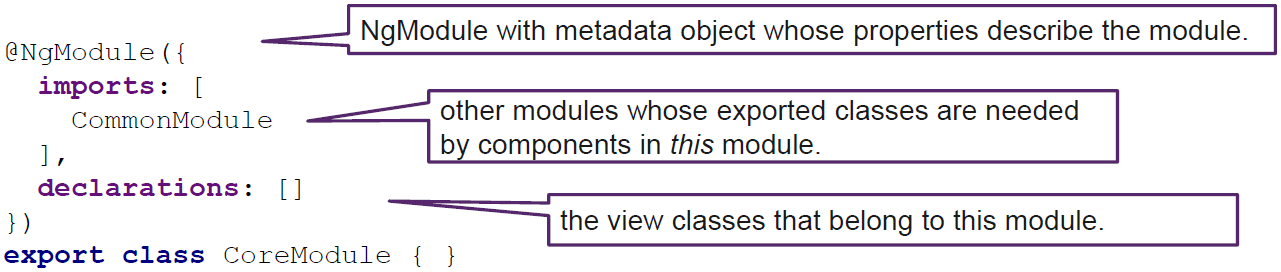
\includegraphics[width=\linewidth]{angular_module_declaration.png}
\textbf{declarations:} View Classes that belong to this module (Components, Directives, Pipes). \textbf{exports:} Subset of declarations that should be visible and usable by other modules. \textbf{imports:} Specifies the modules which exports/providers should be imported. \textbf{providers:} Creators of services that this module contributes to the global collection of services (DI Container). They become accessible in all parts of the app. \textbf{bootstrap:} The main application view, called the root component. Only the root module should set this property.
\subsection{Components}
A Component manages the view and binds data from the model. It consists of:
\begin{itemize}[topsep=0pt, leftmargin=3mm]
    \setlength\itemsep{-0.3em}
    \item Controller $\rightarrow$ provides logic of view, declared as TS-Class with an @component() function decorator
    \item HTML file $\rightarrow$ declares visual interface (template expression)
    \item (S)CSS file $\rightarrow$ styles behind HTML file
\end{itemize}
\textbf{Components} can be nested (results in a Component tree). Provide intofrmation hiding:
\begin{itemize}[topsep=0pt, leftmargin=3mm]
    \setlength\itemsep{-0.3em}
    \item Each Component declares a part of the UI
    \item A Component should be implemented as small coherent piece to support \textcolor{b}{Testability}, \textcolor{b}{Maintainability}, \textcolor{b}{Reusability}
\end{itemize}
Components must be declared within the containing module so its \textbf{selector} is registered for all sub-components of that module. They can be exported, so other modules can import them.
\textcolor{b}{\textbf{Components Lifecycle:}} Most important events are create (ngOnInit) and destroy (ngOnDestroy). ngAfter\ldots events are mainly for control.
\subsection{Templates}
Angular extends the HTML vocabulary of your templates with: Interpolation ( $\{\{$\ldots$\}\}$ ), Template Expression/Statements, Binding Syntax, Directives, Template Reference Variables, Template Expression Operators\\
\textcolor{b}{\textbf{Binding:}}
\begin{lstlisting}[style=htmlcssjs]
// Two Way Binding / Banana in a box [( ... )]
<input type="text" [(ngModel)]="counter.team">
// One Way (from View to Model / Event Binding) ( ... )
<button (click)="counter.eventHandler($event)">
//OneWay (Model to View/Property Binding) [..] or {{..}}
<p>... {{counter.team}} ..</p>
<img [attr.alt]="counter.team" src="team.jpg">
\end{lstlisting}
Binding to targets must be declared as Inputs or Outputs. Targets stands on the left side of the binding declaration
\subsection{Directives}
Similar to a component, but without a template. TypeScript class with an \textit{@Directive()} function decorator.\\
\textcolor{b}{\textbf{Attribute Directives:}} Changes the appearance or behavior of an element, component, or another directive. Applied to a host element as an attribute (eg: ngStyle, ngClass). Does not change the DOM. \textcolor{b}{\textbf{Structural Directives:}} Reshape the DOM's structure, typically by adding, removing, or manipulating elements. Applied to a host element as an attribute (eg: *ngIf, *ngFor)\\
\textcolor{b}{\textbf{Template Reference Variables:}}
\begin{lstlisting}[style=htmlcssjs]
<input placeholder="phone number" #phone>
// phone refers to the input element; pass its `value` to an event handler
<button (click)="callPhone(phone.value)">Call</button>
\end{lstlisting}
\subsection{Services}
Provides any value, function, or feature that your application needs. Typical services are: logging service, data service, message bus, tax calculator, application configuration
\begin{lstlisting}[style=htmlcssjs]
@Injectable({ providedIn: 'root' })
export class CounterService { ... }
\end{lstlisting}
\subsection{Forms}
An Angular form coordinates a set of data-bound user controls. $\rightarrow$ tracks changes, validates input and presents errors. Angular Forms is an external, optional Angular NgModule called FormsModule. Two ways to build: Template-driven, Reactive Forms
\subsection{Asynchronous Services}
Services contain major application logic. Interact with the data resources in an async manner. \textbf{Two options:}\\
1. RxJS can be used to reduce async data managmt complexity.\\
2. EventEmitter class to notify components about data updates.
\subsection{Data Access}
\textcolor{b}{\textbf{HTTP Client}} implements asynchronisms by using the RxJS library (library that implements the Observable pattern).\\
\textbf{Hot Observables:} Sequence of events (mouse move), shared among all subscribers \textbf{Cold Observables:} start running on subscription (async web requests), Not shared among subscribers, automatically closed after task is finished
\subsection{Routing}
To navigate among the views. Multiple directives: \textcolor{b}{RouterOutlet, RouterLink, RouterLinkActive}\\
\textbf{.forRoot():} use exactly once to declare routes on root level \textbf{.forChild():} use when declaring sub-routings
\begin{lstlisting}[style=htmlcssjs]
const appRoutes: Routes = [ // first-match-wins strategy
  // matches /hero/42, 42 saved in param
  {path: 'hero/:id', component: 'Hero'},
  // redirect
  {path: '', redirectTo: '/heroes', pathMatch: 'full'},
  {path: '**', component: PageNotFound} ]; // Wildcard
//Lazy Loading
{path: 'config', loadChildren: () => import('./cfg/cfg
.module').then(m => m.CfgModule), canLoad: [AuthGuard] }
\end{lstlisting}
\subsection{Redux Architecture}
\textbf{ngrx:} implements the Redux pattern using RxJS.
\textbf{Benefits:}
\begin{itemize}[topsep=0pt, leftmargin=3mm]
    \setlength\itemsep{-0.3em}
    \item Enhanced debugging, testability and maintainability
    \item Undo/redo can be implemented easily
    \item Reduced code in Angular Components
\end{itemize}
\textbf{Liabilities:}
\begin{itemize}[topsep=0pt, leftmargin=3mm]
    \setlength\itemsep{-0.3em}
    \item Additional 3rd party library required
    \item More complex architecture
    \item Lower cohesion, global state may contain UI / business data
    \item Data logic may be fragmented into multiple effects/reducers
\end{itemize}